\documentclass{beamer}
\usetheme[pageofpages=de,% String used between the current page and the
                         % total page count.
          bullet=circle,% Use circles instead of squares for bullets.
          titleline=true,% Show a line below the frame title.
          alternativetitlepage=true,% Use the fancy title page.
          titlepagelogo=../img/fse_ministerio_ancho_texto.png%,% Logo for the first page.
	  %watermark=junta_girado,
          %watermarkheight=75px,% Height of the watermark.
          %watermarkheightmult=4,% The watermark image is 4 times bigger
                                % than watermarkheight.
          ]{Torino}

\usepackage[spanish]{babel} % Para separar correctamente las palabras
\usepackage[utf8]{inputenc} % Este paquete permite poner acentos y eñes usando codificación utf-8

\usepackage{color}

\author{IES Gonzalo Nazareno\\
IES Los Albares\\
IES La Campiña\\
IES Ingeniero de la Cierva}
\title{Introducción a Horizon}
\institute{Proyecto de Innovación\\ {\color{white} .\\} \emph{Implantación y puesta a punto de la infraestructura de un cloud 
computing privado para el despliegue de servicios en la nube}}


\begin{document}
\begin{frame}[t,plain]
\titlepage
\end{frame}

\begin{frame}
  \frametitle{Horizon}
  \begin{itemize}
  \item Horizon es el panel de control web (\textit{dashboard}) de OpenStack
  \item Es una aplicación web desarrollada en Django
  \item Implementa las funcionalidades básicas de los componentes principales de OpenStack: Nova, Glance, Swift, etc.
  \item Permite utilizar fácilmente OpenStack mediante una interfaz web simple
  \item Como todos los componentes de OpenStack está sometida a un fuerte desarrollo y varía mucho de una versión a la siguiente
  \item Aquí mostraremos la utilización en OpenStack Essex
  \end{itemize}
\end{frame}

\begin{frame}
  \frametitle{Acceso a Horizon}
  \begin{columns}
    \column{.7\textwidth}
    \begin{itemize}
    \item Acceso mediante usuario/contraseña
    \item Dos roles predefinidos: admin y member
    \item Un usuario con el rol member puede:
      \begin{itemize}
      \item Crear instancias
      \item Modificar el estado de sus instancias
      \item Adquirir direcciones IP públicas
      \item Asociar direcciones IP públicas a sus instancias
      \item Crear y editar reglas de acceso a sus instancias mediante los Grupos de Seguridad
      \item Crear pares de clave ssh y asociarlas a instancias
      \end{itemize}
    \end{itemize}
    \column{.3\textwidth}
    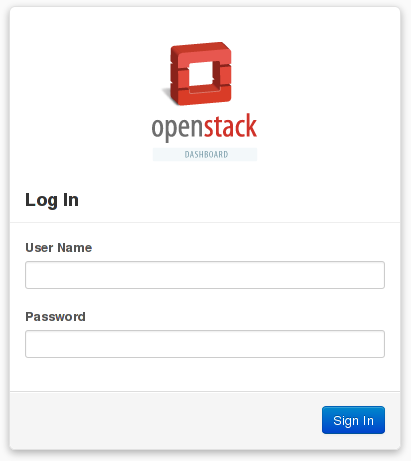
\includegraphics[width=\columnwidth]{../img/horizon1.png}
  \end{columns}
\end{frame}

\begin{frame}
  \frametitle{Conceptos previos}
  \begin{description}
  \item[Imagen] Imagen de sistema preconfigurado que se utiliza como base para crear instancias. Dentro del cloud habrá diferentes imágenes para cada tipo de instacia que se quiera utilizar.
  \item[Instancia] Clon de una imagen que se crea a demanda del usuario en uno de los nodos del cloud. 
  \item[IP privada] Dirección IP con la que se crean las instancias y que se utiliza para comunicación interna.
  \item[IP flotante] Dirección IP pública que puede asociarse a diferentes instancias con el fin de acceder a ellas desde fuera.
  \item [Grupo de seguridad] Reglas de cortafuegos (iptables) que controlan el acceso a las instancias mediante la dirección IP flotante. 
  \item[Par de claves ssh] Utilizadas para acceder por ssh a las instancias desde fuera del cloud. Durante el inicio de la instancia se le ``inyecta'' la clave pública que se indique.
  \end{description}
\end{frame}

\begin{frame}
  \frametitle{Acceso inicial}
  \begin{columns}
    \column{.5\textwidth}
    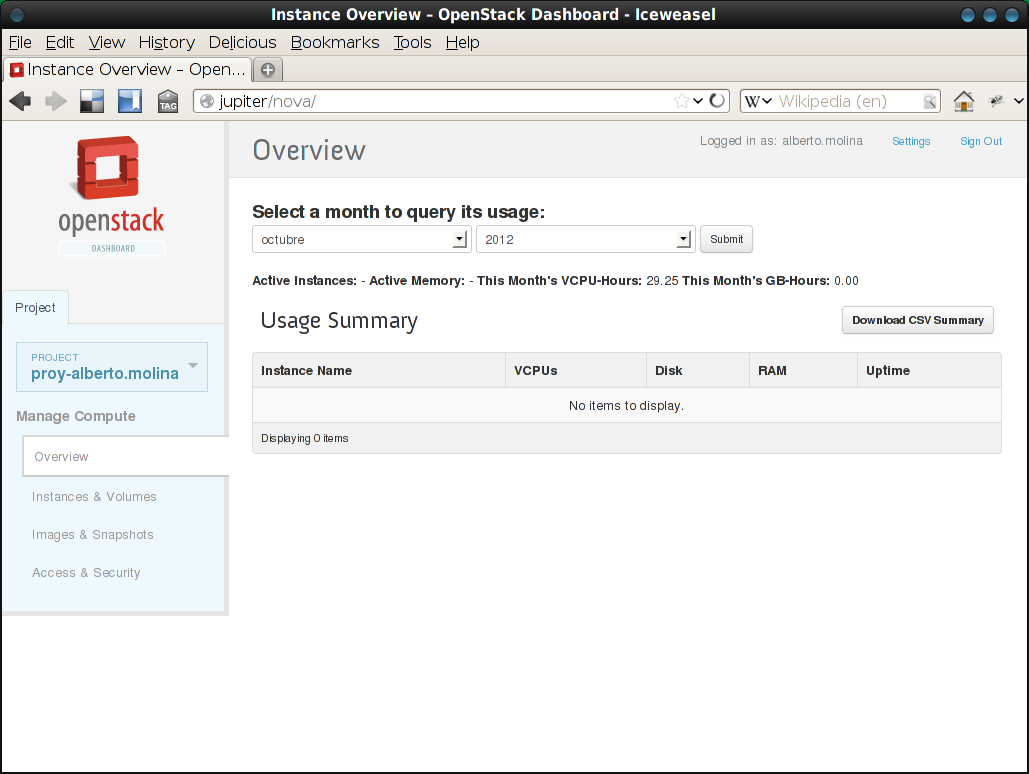
\includegraphics[width=\columnwidth]{../img/horizon2.png}    
    \column{.5\textwidth}
    \begin{itemize}
    \item Un usuario puede pertenecer a diferentes proyectos
    \item Sencillo menú que muestra las acciones a realizar
    \end{itemize}
  \end{columns}
\end{frame}

\begin{frame}
  \frametitle{Grupo de Seguridad}
  \begin{itemize}
  \item Es posible definir diferentes grupos de seguridad (conjunto de reglas de cortafuegos) para aplicar a las instancias de cada proyecto.
  \item 
  \end{itemize}
\end{frame}
\end{document}
